%-----------------------------------------------------------------------------
%
%               Template for sigplanconf LaTeX Class
%
% Name:         sigplanconf-template.tex
%
% Purpose:      A template for sigplanconf.cls, which is a LaTeX 2e class
%               file for SIGPLAN conference proceedings.
%
% Guide:        Refer to "Author's Guide to the ACM SIGPLAN Class,"
%               sigplanconf-guide.pdf
%
% Author:       Paul C. Anagnostopoulos
%               Windfall Software
%               978 371-2316
%               paul@windfall.com
%
% Created:      15 February 2005
%
%-----------------------------------------------------------------------------


\documentclass[preprint]{sigplanconf}

% The following \documentclass options may be useful:

% preprint      Remove this option only once the paper is in final form.
% 10pt          To set in 10-point type instead of 9-point.
% 11pt          To set in 11-point type instead of 9-point.
% authoryear    To obtain author/year citation style instead of numeric.

\usepackage{amsmath}
\usepackage{graphicx}
\usepackage{hyperref}

\begin{document}

\special{papersize=8.5in,11in}
\setlength{\pdfpageheight}{\paperheight}
\setlength{\pdfpagewidth}{\paperwidth}

\conferenceinfo{Workshop on Programming Models for SIMD/Vector Processing '14}{February, 2014, Orlando, FL, USA} 
\copyrightyear{2014} 
\copyrightdata{978-1-nnnn-nnnn-n/yy/mm} 
\doi{nnnnnnn.nnnnnnn}

% Uncomment one of the following two, if you are not going for the 
% traditional copyright transfer agreement.

%\exclusivelicense                % ACM gets exclusive license to publish, 
                                  % you retain copyright

%\permissiontopublish             % ACM gets nonexclusive license to publish
                                  % (paid open-access papers, 
                                  % short abstracts)


\title{A SIMD Programming Model for Dart, JavaScript, and other dynamically typed scripting languages}

\authorinfo{John McCutchan}
           {Google}
           {johnmccutchan@google.com}
\authorinfo{Haitao Feng}
           {Intel}
           {haitao.feng@intel.com}

\maketitle

\begin{abstract}
It has not possible to take advantage of the SIMD coprocessors available in all x86 and most ARM processors shipping today in dynamically typed scripting languages. Web browsers have become a mainstream platform to deliver large and complex applications with feature sets and performance comparable to native applications, programmers must choose between Dart and JavaScript when writing web programs. This paper introduces an explicit SIMD programming model for Dart and JavaScript, we show that it can be compiled to efficient x86/SSE or ARM/NEON code by both Dart and JavaScript virtual machines achieving a 300\%-600\% speed increase across a variety of benchmarks. The result of this work is that more sophisticated and performant applications can be built to run in web browsers. The ideas introduced in this paper can also be used in other dynamically typed scripting languages to provide a similarly performant interface to SIMD coprocessors.
\end{abstract}

\section{Introduction}
All x86 and many ARM processors shipping today include a dedicated single instruction multiple data (SIMD) coprocessor.  On x86 the SSE instruction set allows for computing on 128-bit wide registers. ARM has the NEON instruction set which allows for computing on 128-bit wide registers. Both SSE and NEON have instructions for computing on 4 single precision floating point numbers (Float32x4) and 4 signed integers (Int32x4) stored in 128-bit registers. There are also instructions available for operating on 2 double precision floating point numbers (Float64x2) as well as algorithm specific instructions for operating on sound or pixel data.

Web browsers as a platform to deliver complex applications with feature sets and performance that are comparable to native desktop applications has become mainstream. All major browsers (Chrome, Firefox, Safari, and IE) include support for displaying 3D graphics through WebGL, playing 3D positional audio through WebAudio. These applications are written directly in JavaScript, Dart, or compiled to JavaScript from C/C++ code through the LLVM based emscripten\cite{emscripten} compiler. Starting in 2008 with the advent of the V8 JavaScript virtual machine (VM) performance of JavaScript execution has increased dramatically with browser vendors competing for the fastest JavaScript VM. Dart is a new web programming language designed for performance with a custom VM.

Despite the dramatic increase in performance it has not been possible for web programs to access the dedicated SIMD coprocessors. JavaScript is limited to scalar operations on double precision floating point values and Dart is limited to scalar operations on double precision floating point values and integers. In this paper we introduce:

\begin{itemize} 
\item A SIMD programming model for Dart and JavaScript languages. The programming model is high level but allows for explicit control over the SIMD coprocessors. It supports comparisons, branchless selection based on comparison results, and efficient shuffling of scalar values within a SIMD value. The programming model does not rely on compiler optimization passes like auto vectorization. 
\item Three (Float32x4, Int32x4, and Float64x2) new numeric value types for Dart and JavaScript.
\item Efficient array storage of the new numeric value types.
\item How we generate performant machine code that is free of high level abstraction in Dart and JavaScript VMs.
\item An implementation of the programming model for the Dart VM that has shipped and is used in production today.
\item An implementation of the programming model for the V8 JavaScript VM.
\item Benchmarks that show (depending on the algorithm) a speedup of 300-600\% across problem domains including real-time 3D graphics, numerical computation, ray tracing, and cryptography.
\end{itemize}

\section{Lack of SIMD programmability for web applications}
Many algorithms can be sped up by taking advantage of SIMD coprocessors. A simple example is the averaging of an array of numbers. The scalar algorithm, in Dart:

\begin{verbatim} 
double average(Float32List data) {
  var sum = 0.0;
  for (var i = 0; i < data.length; i++) {
    sum += data[i]; 
  }
  return sum / data.length;
}
\end{verbatim}

The algorithm simply accumulates all the data points and computes the average by dividing by the number of data points. This algorithm can trivially take advantage of SIMD coprocessors by adding 4 numbers at the same time. The SIMD algorithm, in Dart:

\begin{verbatim}
double average(Float32x4List data) {
  var sum = new Float32x4.zero();
  for (var i = 0; i < data.length; i++) {
    sum += data[i];
  }
  var total = sum.x + sum.y + sum.z + sum.w;
  return total / (data.length * 4);
}
\end{verbatim}

The bulk of the work is done in parallel and only after the exiting the loop does the program need to fall back to scalar computation when computing the final sum and average.

If the Float32x4 type were available to web programmers and the optimizing compiler is successful in generating code that is free of memory allocation and allows for temporary values to stay in CPU registers, the algorithm can be sped up by 500\%. In the following section, we provide more details on the programming model and how it can be efficiently compiled for x86 and ARM processors.

\section{Bringing SIMD to the Web}
The SIMD programming model for Dart and JavaScript is designed to give direct control to the programmer (or the Dart or C++ compiler generating JavaScript). It introduces three new 128-bit wide value types: Float32x4, Int32x4, and Float64x2. Each value type stores scalar values in multiple "lanes". For example, Float32x4 has four single precision floating point numbers in lanes labelled: x, y, z, and w. Note that w is the fourth lane and not the first. Each instance is immutable and all operations result in a new instance.

\subsection{Primitive Operations}
This section will focus on the Float32x4 type. The other types offer similar operations but can be limited by a lack of actual instructions in SSE or NEON. For example, there is no Int32x4 divide instruction in either SSE or NEON instruction sets. Emulation of missing instructions is discussed in future work.

Float32x4 supports standard arithmetic operations (+, -, *, /) as well as approximate square root, reciprocal square root, and reciprocal. It also supports absolute value, minimum, maximum, and clamp operations. All of these operations are performed for each lane. For example, the minimum value of two Float32x4 is the Float32x4 with the minimum value of each individual lane.

\subsection{Type Conversion}
Value cast operations between Float32x4 and Int32x4 as well as Float32x4 and Float64x2 are available. In the conversion between Float32x4 and Float64x2 only the x and y lanes are used.

Bit-wise cast operations between Float32x4, Int32x4, and Float64x2 are available. These do not interpret the lane values but provide a mechanism to directly convert the 128-bit value between all type pairs. 

\subsection{Comparison and Branchless Selection}
When comparing SIMD values the result is not a single boolean value but a boolean value for each lane. Consider the example of computing the minimum value of two values. The scalar algorithm, in Dart:
\begin{verbatim}
num min(num a, num b) {
  if (a <= b) {
    return a;
  }
  return b;
}
\end{verbatim}

The lane-wise SIMD algorithm, in Dart:

\begin{verbatim}
Float32x4 min(Float32x4 a, Float32x4 b) {
  Int32x4 mask = a.lessThanOrEqual(b);
  return mask.select(a, b);
}
\end{verbatim}

The comparison results in an Int32x4 value with lanes containing 0xFFFFFFFF or 0x0 when the lane comparison is true or false respectively. The resulting mask is used to pick which value's lane should be used. 

\subsection{Lane Access and Shuffling}
Direct access of each lane of a Float32x4 can be had by accessing the x, y, z, or w instance properties. An example of this is shown in the average algorithm. Shuffling the order of lanes can also be done. Reversing the order of the lanes, in Dart:
\begin{verbatim}
Float32x4 reverse(Float32x4 v) {
  return v.shuffle(Float32x4.WZYX);
}
\end{verbatim}

The shuffle method uses an integer mask to reorder the lane values in v. All 256 combinations are supported.

Because each instance is immutable it is not possible to change the value stored in one of the values lanes. Methods, for example, \verb!withX! allow for constructing new instances that are copies of an existing instance with an individual lane value changed. In example, in Dart:

\begin{verbatim}
var x = new Float32x4(1.0, 2.0, 3.0, 4.0);
var y = x.withX(5.0);
\end{verbatim}

\subsection{Memory I/O}
Up until this point we have only discussed individual values but in order to be a generally useful programming model, compact and cache-friendly array storage of each type is introduced. Float32x4List, Int32x4List, and Float64x2List offer contiguous storage of Float32x4, Int32x4, and Float64x2 values. Loading and storing, in Dart:

\begin{verbatim}
void copy(Float32x4List destination, Float32x4List source,
	          int n) {
  for (var i = 0; i < n; i++) {
    var x = source[i];   // Load.
    destination[i] = x;  // Store.
  }
}
\end{verbatim}

Note that on load a new instance of Float32x4 is constructed. In sections \ref{boxing} and \ref{inlining} we discuss how the memory allocation and instance construction is avoided in optimized code.

\subsection{Mapping from high level to low level}
The programming model is high level with each operation requiring a method call on a heap allocated object and results in a new heap allocated object holding the resulting value. Each value is immutable and storage of temporary values cannot be reused. The design of the programming model was done with care so that when optimized code is generated, the overhead of the high level programming model can be removed. Almost all method calls will be mapped directly to a single CPU instruction. Some operations require slightly longer instruction sequences but so would a hand written assembly programming performing the same operation. Instances will be stored directly inside CPU registers avoiding the cost of memory allocation and object creation. The following section covers how this is accomplished.

\section{Dart VM and V8 implementation}
We will now discuss the implementation details of the programming model in the Dart VM. Section \ref{V8} discusses the implementation for the V8 VM.

\subsection{Unoptimized Code}
When a function is first compiled by the Dart VM the generated code is completely generic. Every method call is looked up in the receiving object's class's function table. Every temporary value is allocated in the heap as a full object under control of the GC. 

\subsection{Type Collection}
The unoptimized code collects important type\cite{typefeedback} information that is used later by the optimizing compiler. At each method call the unoptimized code maintains a cache mapping from receiver class id to address of the function. 

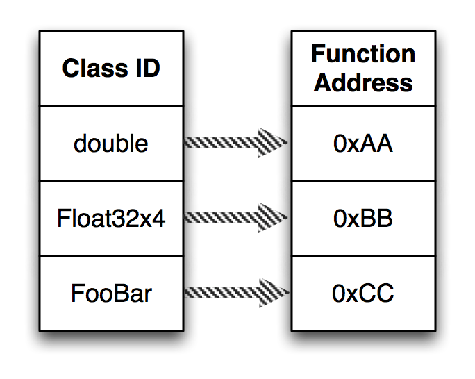
\includegraphics{typecache.eps}
This data has two important uses:
\begin{itemize}
\item Future execution of the unoptimized code will be faster if the receiving object has a class id already seen at the call site. Execution is faster because looking up the function for the method on the receiving object will result in a cache hit, avoiding the expensive lookup and cache update.
\item Types seen at a method call site are fed into the optimizing compiler and code that optimistically expects to see the same type can be generated.
\end{itemize}

\subsection{Boxed and Unboxed Values}

\label{boxing}
The Dart compiler makes a distinction between boxed and \\
unboxed\cite{unboxing} values. Boxed values are pointers to objects which are allocated in the heap whose life cycle is managed by the GC. Unboxed values are stored in CPU registers. Operations on unboxed values are much more efficient because the values are already contained in CPU registers. An instance of Float32x4 looks like:


\includegraphics{boxedobject.eps}

The object header contains information used for type collection and the GC.

\subsection{Parameter Passing}
The Dart VM passes all method parameters and the return value as boxed instances. This can have a negative performance impact as unboxed values will be boxed for the method call which will immediately unbox them again.

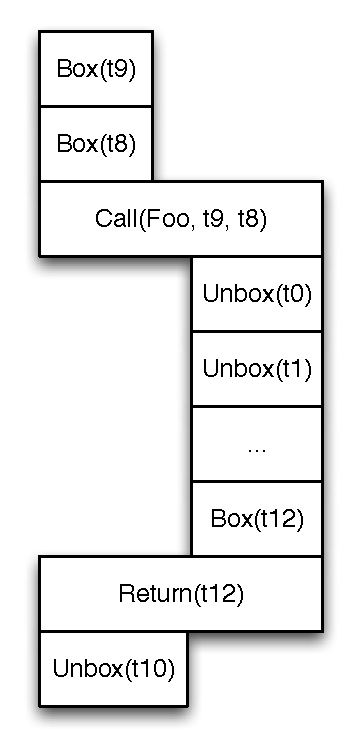
\includegraphics{boxunboxbox.eps}

\subsection{Inlining}
\label{inlining}
Both the Dart VM and V8 make heavy use of inlining to avoid method call invocation and unnecessary boxing of values. The first form of inlining is similar to the inlining done in many compilers, the bodies of small functions are copied into the calling function, replacing the method call. The second form of inlining, replacement of runtime provided functions with compiler intermediate representation (IR) instructions is the key to achieving high performance with this programming model. Consider the following code, in Dart:

\begin{verbatim}
Float32x4 compute(Float32x4 a, Float32x4 b) {
  var c = a + b;
  var d = a * a;
  var e = b *  b;
  return c + d + e;
}
\end{verbatim}

In unoptimized code, the compiled pseudo code:

\begin{verbatim}
t0 <- Call(+, a, b);
t1 <- Call(*, a, a);
t2 <- Call(*, b, b);
t3 <- Call(+, t0, t1);
t4 <- Call(+, t3, t2);
return t4;
\end{verbatim}

So long as the function \verb!compute! has only ever been given Float32x4 instances, the compiler will recognize all of the call sites are monomorphic, in other words, each call site has a single receiver class id and target function. The type data collected in unoptimized code at each method call site is used to determine whether this is the case or not. The function targets \verb!Float32x4_Add! and \verb!Float32x4_Mul! are both provided by runtime and the compiler knows how to replace them with IR instructions. As mentioned above, the functions only accept and return boxed instances but the Float32x4 IR instructions only accept and return unboxed values. 

\subsection{Optimized Code}
When inlining is successful the optimized code will be free of object construction and method call invocations. Consider the following function, in Dart:

\begin{verbatim}
Float32x4 compute(Float32x4 a, Float32x4 b) {
  var c = a + b;
  var d = a * a;
  var e = b *  b;
  return c + d + e;
}
\end{verbatim}

The pseudocode of the above function when optimized:

\begin{verbatim}
if (!TypeMatch(a, Float32x4)) {
  deoptimize();
}
if (!TypeMatch(b, Float32x4)) {
  deoptimize();
}
t0 <- unbox(a);
t1 <- unbox(b);
t2 <- BinaryFloat32x4Op+(t0, t1);
t3 <- BinaryFloat32x4Op*(t0, t0);
t4 <- BinaryFloat32x4Op*(t1, t1);
t5 <- BinaryFloat32x4Op+(t2, t3);
t6 <- BinaryFloat32x4Op+(t5, t4);
return box(t6);
\end{verbatim}

The optimized code first validates the class of each input value. If any of the types do not match the expected type, the function is deoptimized. For more details on deoptimization see Section \ref{deoptimizing}. After being validated the values are unboxed directly into CPU registers (tN) and the remaining operations are performed directly in CPU registers with no memory I/O. The final step is to box the result so it can be returned.

Under the Dart VM the generated SSE code:

\begin{verbatim}
        ;; CheckClass:14(v2)
0x107822533 testb rdx,0x0x1
0x107822536 jz 0x107822607
0x10782253c movzxwq rbx,[rdx+0x1]
0x107822541 cmpl rbx,0x37
0x107822544 jnz 0x107822607
        ;; CheckClass:14(v3)
0x10782254a testb rcx,0x0x1
0x10782254d jz 0x107822612
0x107822553 movzxwq rbx,[rcx+0x1]
0x107822558 cmpl rbx,0x37
0x10782255b jnz 0x107822612
        ;; v11 <- UnboxFloat32x4:14(v2)
0x107822561 movups xmm1, [rdx+0x7]
        ;; v14 <- UnboxFloat32x4:14(v3)
0x107822565 movups xmm2, [rcx+0x7]
        ;; ParallelMove xmm3 <- xmm1
0x107822569 movaps xmm3, xmm1
        ;; v4 <- BinaryFloat32x4Op:14(+, v11, v14)
0x10782256c addps xmm3, xmm2
        ;; ParallelMove xmm4 <- xmm1
0x10782256f movaps xmm4, xmm1
        ;; v5 <- BinaryFloat32x4Op:26(*, v11, v11)
0x107822572 mulps xmm4, xmm1
        ;; ParallelMove xmm1 <- xmm2
0x107822575 movaps xmm1, xmm2
        ;; v6 <- BinaryFloat32x4Op:38(*, v14, v14)
0x107822578 mulps xmm1, xmm2
        ;; v7 <- BinaryFloat32x4Op:50(+, v4, v5)
0x10782257b addps xmm3, xmm4
        ;; v8 <- BinaryFloat32x4Op:58(+, v7, v6)
0x10782257e addps xmm3, xmm1
        ;; v15 <- BoxFloat32x4:112(v8)
0x107822581 movq r11,[r15+0x47]
0x107822588 movq rax,[r11]
0x10782258b addq rax,0x20
0x10782258f movq r11,[r15+0x4f]
0x107822596 cmpq rax,[r11]
0x107822599 jnc 0x1078225eb
0x10782259f  movq r11,[r15+0x47]
0x1078225a6 movq [r11],rax
0x1078225a9 subq rax,0x1f
0x1078225ad movq [rax-0x1],0x370200
0x1078225b5 movups [rax+0x7], xmm3
\end{verbatim}

For readers unfamiliar with SSE, the following list describes the instructions as used in the above code:
\begin{itemize}
\item \textbf{movups} Unaligned load or store of 128-bit value.
\item \textbf{movaps} Register move.
\item \textbf{addps} Add 4 single precision floating point numbers.
\item \textbf{mulps} Multiply 4 single precision floating point numbers.
\end{itemize}

\subsection{Register Allocation}
The Dart VM already supported unboxed double values which on x86 used the xmm registers. The xmm registers are also needed for Float32x4, Int32x4, and Float64x2 values. The register allocator was extended to support both 8 and 16 byte values stored in xmm registers as well as allocate the appropriate range of memory to spill values from registers to the stack when register pressure requires spilling.

\subsection{Alignment}
SIMD instruction sets provide preferred memory I/O instructions that require the memory address to be aligned on 16-byte boundaries. These instructions are typically faster than the unaligned memory I/O instructions. All memory I/O instructions emitted by the Dart VM are for unaligned addresses because the Dart VM GC cannot guarantee object alignment.

\subsection{Deoptimization}
\label{deoptimizing}
After a function has been optimized if one of the values it uses violates the optimistic type expectations, a deoptimization occurs resulting in the following process:

\begin{itemize}
\item Execution of optimized code stops.
\item Optimized code is invalidated and disconnected from the function.
\item Live unboxed values are boxed.
\item Pointers to boxed values are stored in the correct locations of the unoptimized codes stack frame.
\item Execution of the function's unoptimized code begins at exactly the same point that the deoptimization occurred.
\end{itemize}

An important thing to understand is that only functions which are provided stable input types will be optimized. 

\subsection{Implementation for JavaScript and V8}
\label{V8}
The SIMD programming model for Dart is used for JavaScript as well. The 128-bit wide value types are introduced, but as there are no class and operator overloading language features in JavaScript, the syntax of the SIMD API is different than Dart's. We introduced a SIMD global module with operations grouped by type. The following example demonstrates the syntactic difference. Consider the following programming, in Dart:

\begin{verbatim}
Float32x4 compute(Float32x4 a, Float32x4 b) {
  var c = a + b;
  var d = a * a;
  var e = b *  b;
  return c + d + e;
}
\end{verbatim}

The above program would be written as follows, in JavaScript:

\begin{verbatim}
compute(var a, var b) {
  var c = SIMD.float32x4.add(a, b);
  var d = SIMD.float32x4.mul(a, a);
  var e = SIMD.float32x4.mul(b, b);
  var t = SIMD.float32x4.add(c, d);
  return SIMD.float32x4.add(t, e);
}
\end{verbatim}

The V8 implementation is conceptually similar to the implementation in the Dart VM:
\begin{itemize}
\item We added the 128-bit wide value constructor and SIMD API into full-codegen which generates un-optimized code and optimized them in the Crankshaft which generates optimized code. 
\item We allocated the 128-bit value in a heap object (with a header to indicate the type) and garbage collect it when it is boxed; when the value is un-boxed, we allocate it into a hardware 128-bit register (XMM register in the Intel IA32 and X64 architectures). 
\item We inlined all the SIMD operations, inlining is the key technique for the performance acceleration.
\item Like the Dart VM, when transitioning from optimized to unoptimized code (due to a deoptimization event) the unboxed values are boxed and pointers to the boxed values are placed in the unoptimized codes stack frame.
\end{itemize}

Despite the many similarities, there are some important differences in the V8 implementation:
\begin{itemize}
\item The unoptimized code does not collect type information for Float32x4, Int32x4, and Float32x4 instances. Instead upon entry to a SIMD.type.op function the types of the parameters are verified to match the expected type. If they do not an exception is thrown.
\item Because JavaScript is more dynamic than Dart and allows for object fields and functions to be modified at runtime, for example, the SIMD.float32x4.add method could have been overridden by the program. More checks are required to ensure that these operations have not been replaced with user written code. When this occurs inlining cannot be performed and performance suffers.
\end{itemize}
\section{Benchmarks}
In this section we will present benchmark results for four different benchmarks:
\begin{itemize}
\item \textbf{Average} Averaging many floating point numbers.
\item \textbf{Mandelbrot} Generating a Mandelbrot\cite{mandelbrot} visualization.
\item \textbf{MatrixMultiply} 4x4 matrix multiplication.
\item \textbf{VectorTransform} 3D vertex transformation used for 3D rendering.
\end{itemize}

The benchmarks were run on Ubuntu 13.04 64-bit Linux with Intel CPU (Intel(R) Core(TM) i7-2600 CPU @ 3.40GHz). Full source code of all benchmarks can be obtained at \href{https://github.com/johnmccutchan/ecmascript_simd/}{ECMAScript SIMD Polyfill}. Benchmark results are given as the relative performance gain compared with scalar code in the same language.

\subsection{Dart VM}
\begin{tabular}{|l|r|}
\hline
 Average & 8.5x \\
 \hline
 Mandelbrot & 2.6x \\
 \hline
 MatrixMultiply & 3.9x \\
 \hline
 VectorTransform & 4.9x \\
 \hline
\end{tabular}

\subsection{V8}
\begin{tabular}{|l|r|}
\hline
 Average & 6.1x \\
 \hline
 Mandelbrot & 3.8x \\
 \hline
 MatrixMultiply & 3.8x \\
 \hline
 VectorTransform & 4.2x \\
 \hline
\end{tabular}

\subsection{Discussion}
The benchmark data shows a significant speedups across a variety of algorithms. Some of the results need further explanation. 

Averaging many floating point numbers shows an 850\% speed increase in Dart and a 610\% speed increase in JavaScript. At first this might seem impossible, the theoretical performance gain from SIMD should only be 400\%. It is important to note that in the case of Dart and JavaScript that the scalar code is performing double precision arithmetic where as the SIMD code is performing single precision. The data is being loaded from an array holding single precision floating point values resulting in the scalar code having to convert from single to double precision before performing the calculation where as the SIMD code can load the values directly.

The Mandelbrot benchmark is only sped up by 260\% in Dart but is sped up by 380\% in JavaScript. The reason for the discrepancy is that the Dart implementation has not fully implemented the necessary inlining optimizations for the Int32x4 type which is used in the Mandelbrot benchmark. 

\section{Related Work}
\subsection{C SSE Intrinsics}
C/C++ compilers offer SIMD intrinsic functions (\verb!xmmintrin.h! and \verb!emmintrin.h!). At compile time these function calls are replaced with a single instruction. Conceptually, the SIMD programming model for Dart and JavaScript is similar but neither Dart nor JavaScript has static type information available at compile time and instead, must rely on run-time type collection (or enforcement) before the compiler can emit the SSE instructions.
\subsection{SIMD in C\#}
The Mono C\# compiler provided an API for SIMD\cite{monosimd} programming. This API is considered experimental and directly mimics the SSE instruction set without any concern for portability across different SIMD instruction sets. The SIMD programming model presented in this paper was designed to run across SSE and NEON instruction sets and has been implemented for both.
\subsection{Auto-Vectorization}
Mozilla has experimented\cite{mozillasimd} with an auto vectorization pass in their JavaScript compiler. The focus of this work was on a gaussian blur algorithm written in JavaScript. Speed gains of approximately 20\% were achieved. This work was never merged and appears abandoned.

\section{Conclusions and Future Work}
In this paper we have presented a high level programming model that offers direct control of SIMD coprocessors to web programs in both Dart and JavaScript. We have shown how both Dart and JavaScript VMs can avoid memory allocation and the resulting garbage collector (GC) pressure by avoiding instance creation with inlining and unboxed values. We have discussed the implementations in both the Dart VM and V8. Finally, we have presented benchmarks demonstrating the real world performance gains that this programming model provides. Future work includes:
\begin{itemize} 
\item Support for wider (256-bit and 512-bit) SIMD register widths (AVX and AVX-512) and the natural data types they offer, for example, Float32x8 and Float32x16. This includes generating correct code for wider register widths on CPUs that only support 128-bit wide registers.
\item Support for pixel processing by developing a portable abstraction around instructions that are algorithm specific operating on 16 individual bytes. Including support for saturating arithmetic operations.
\item Support operations which do not have CPU instructions available, for example, Int32x4 division. 
\item Supporting for passing and returning unboxed values directly, avoiding the overhead of boxing values on method invocation and return.
\item Support types that have few SIMD instructions, for example, Int16x8. Speed ups may be seen on these types because efficient native code can that does N scalar operations can be emitted directly.
\end{itemize}
\bibliographystyle{abbrvnat}

% The bibliography should be embedded for final submission.

\begin{thebibliography}{}
\softraggedright

\bibitem[Urs]{typefeedback}
H\"{o}lzle, Urs and Ungar, David Reconciling Responsiveness with Performance in Pure Object-oriented Languages
\bibitem[Leroy]{unboxing}
Xavier Leroy Unboxed objects and polymorphic typing
\bibitem[Mono C\# SIMD]{monosimd}
\url{http://docs.go-mono.com/?link=N\%3aMono.Simd}
\bibitem[Mozilla Auto Vectorization]{mozillasimd}
\url{https://bugzilla.mozilla.org/show_bug.cgi?id=832718}
\bibitem[Mandelbrot]{mandelbrot}
\url{http://en.wikipedia.org/wiki/Benoit_Mandelbrot}
\bibitem[Emscripten]{emscripten}
\url{http://en.wikipedia.org/wiki/Emscripten}
\end{thebibliography}


\end{document}

%                       Revision History
%                       -------- -------
%  Date         Person  Ver.    Change
%  ----         ------  ----    ------

%  2013.06.29   TU      0.1--4  comments on permission/copyright notices

